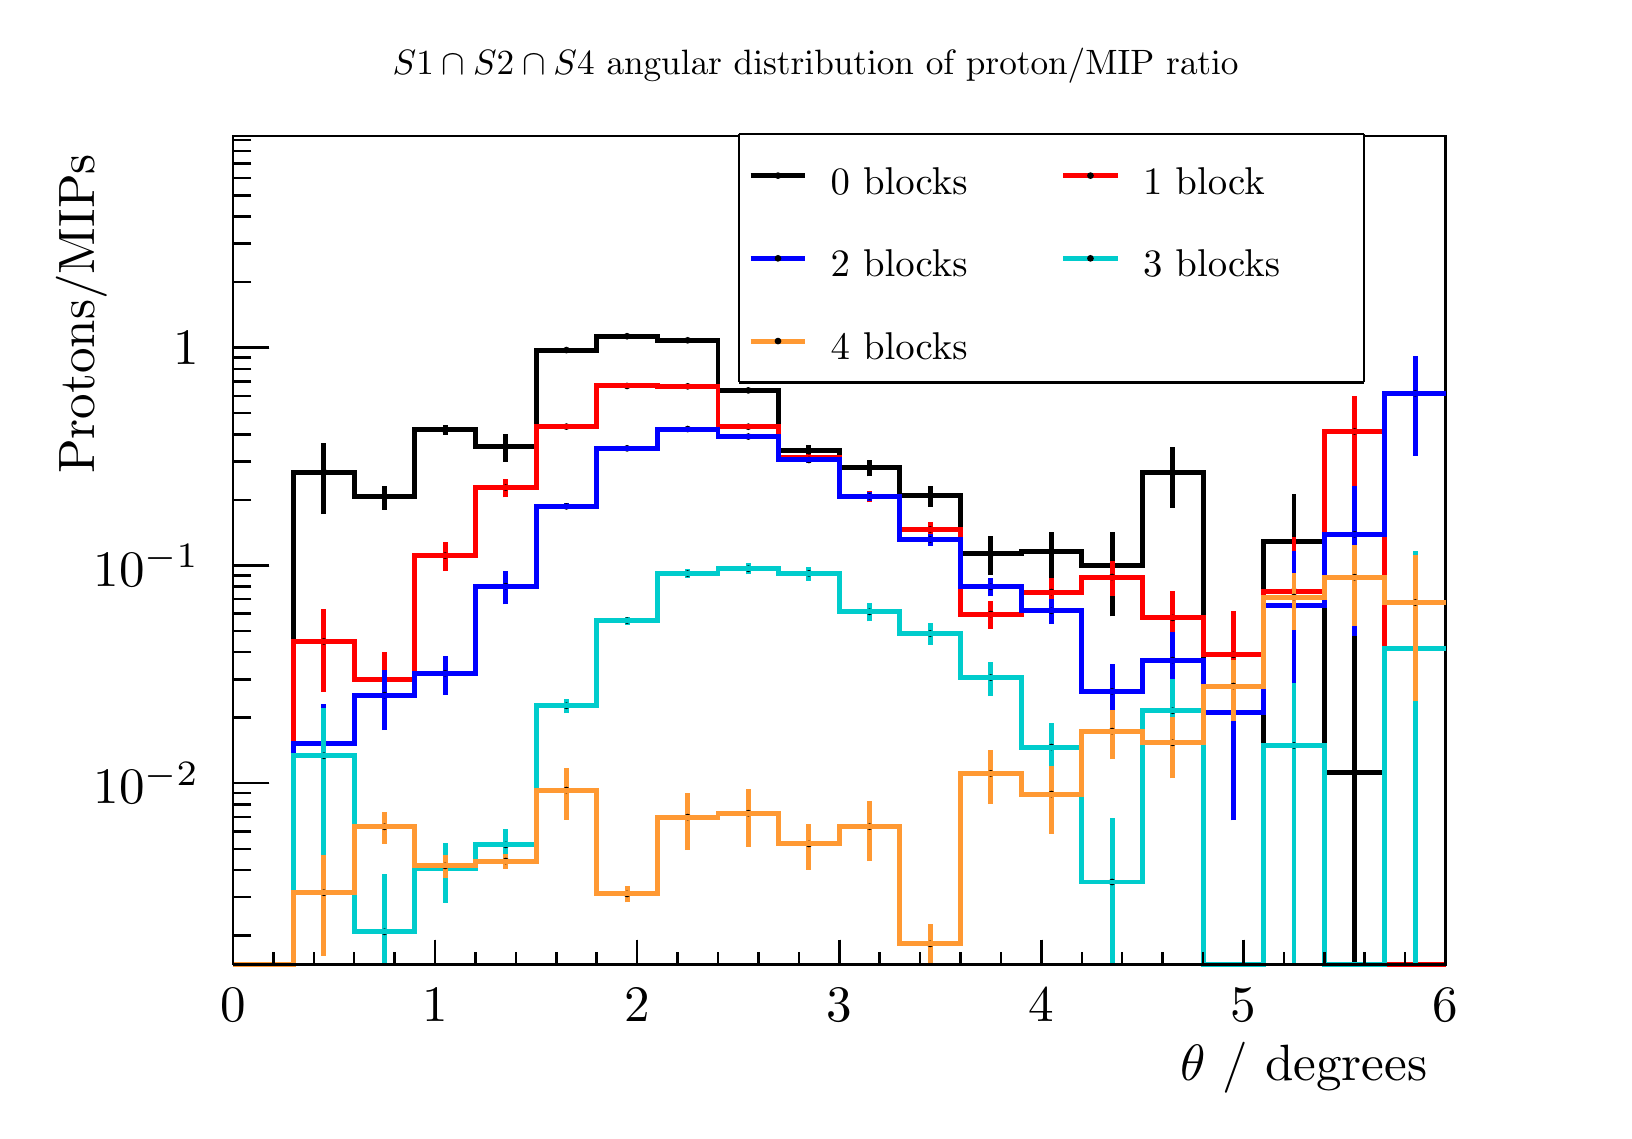
\begin{tikzpicture}
\pgfdeclareplotmark{cross} {
\pgfpathmoveto{\pgfpoint{-0.3\pgfplotmarksize}{\pgfplotmarksize}}
\pgfpathlineto{\pgfpoint{+0.3\pgfplotmarksize}{\pgfplotmarksize}}
\pgfpathlineto{\pgfpoint{+0.3\pgfplotmarksize}{0.3\pgfplotmarksize}}
\pgfpathlineto{\pgfpoint{+1\pgfplotmarksize}{0.3\pgfplotmarksize}}
\pgfpathlineto{\pgfpoint{+1\pgfplotmarksize}{-0.3\pgfplotmarksize}}
\pgfpathlineto{\pgfpoint{+0.3\pgfplotmarksize}{-0.3\pgfplotmarksize}}
\pgfpathlineto{\pgfpoint{+0.3\pgfplotmarksize}{-1.\pgfplotmarksize}}
\pgfpathlineto{\pgfpoint{-0.3\pgfplotmarksize}{-1.\pgfplotmarksize}}
\pgfpathlineto{\pgfpoint{-0.3\pgfplotmarksize}{-0.3\pgfplotmarksize}}
\pgfpathlineto{\pgfpoint{-1.\pgfplotmarksize}{-0.3\pgfplotmarksize}}
\pgfpathlineto{\pgfpoint{-1.\pgfplotmarksize}{0.3\pgfplotmarksize}}
\pgfpathlineto{\pgfpoint{-0.3\pgfplotmarksize}{0.3\pgfplotmarksize}}
\pgfpathclose
\pgfusepathqstroke
}
\pgfdeclareplotmark{cross*} {
\pgfpathmoveto{\pgfpoint{-0.3\pgfplotmarksize}{\pgfplotmarksize}}
\pgfpathlineto{\pgfpoint{+0.3\pgfplotmarksize}{\pgfplotmarksize}}
\pgfpathlineto{\pgfpoint{+0.3\pgfplotmarksize}{0.3\pgfplotmarksize}}
\pgfpathlineto{\pgfpoint{+1\pgfplotmarksize}{0.3\pgfplotmarksize}}
\pgfpathlineto{\pgfpoint{+1\pgfplotmarksize}{-0.3\pgfplotmarksize}}
\pgfpathlineto{\pgfpoint{+0.3\pgfplotmarksize}{-0.3\pgfplotmarksize}}
\pgfpathlineto{\pgfpoint{+0.3\pgfplotmarksize}{-1.\pgfplotmarksize}}
\pgfpathlineto{\pgfpoint{-0.3\pgfplotmarksize}{-1.\pgfplotmarksize}}
\pgfpathlineto{\pgfpoint{-0.3\pgfplotmarksize}{-0.3\pgfplotmarksize}}
\pgfpathlineto{\pgfpoint{-1.\pgfplotmarksize}{-0.3\pgfplotmarksize}}
\pgfpathlineto{\pgfpoint{-1.\pgfplotmarksize}{0.3\pgfplotmarksize}}
\pgfpathlineto{\pgfpoint{-0.3\pgfplotmarksize}{0.3\pgfplotmarksize}}
\pgfpathclose
\pgfusepathqfillstroke
}
\pgfdeclareplotmark{newstar} {
\pgfpathmoveto{\pgfqpoint{0pt}{\pgfplotmarksize}}
\pgfpathlineto{\pgfqpointpolar{44}{0.5\pgfplotmarksize}}
\pgfpathlineto{\pgfqpointpolar{18}{\pgfplotmarksize}}
\pgfpathlineto{\pgfqpointpolar{-20}{0.5\pgfplotmarksize}}
\pgfpathlineto{\pgfqpointpolar{-54}{\pgfplotmarksize}}
\pgfpathlineto{\pgfqpointpolar{-90}{0.5\pgfplotmarksize}}
\pgfpathlineto{\pgfqpointpolar{234}{\pgfplotmarksize}}
\pgfpathlineto{\pgfqpointpolar{198}{0.5\pgfplotmarksize}}
\pgfpathlineto{\pgfqpointpolar{162}{\pgfplotmarksize}}
\pgfpathlineto{\pgfqpointpolar{134}{0.5\pgfplotmarksize}}
\pgfpathclose
\pgfusepathqstroke
}
\pgfdeclareplotmark{newstar*} {
\pgfpathmoveto{\pgfqpoint{0pt}{\pgfplotmarksize}}
\pgfpathlineto{\pgfqpointpolar{44}{0.5\pgfplotmarksize}}
\pgfpathlineto{\pgfqpointpolar{18}{\pgfplotmarksize}}
\pgfpathlineto{\pgfqpointpolar{-20}{0.5\pgfplotmarksize}}
\pgfpathlineto{\pgfqpointpolar{-54}{\pgfplotmarksize}}
\pgfpathlineto{\pgfqpointpolar{-90}{0.5\pgfplotmarksize}}
\pgfpathlineto{\pgfqpointpolar{234}{\pgfplotmarksize}}
\pgfpathlineto{\pgfqpointpolar{198}{0.5\pgfplotmarksize}}
\pgfpathlineto{\pgfqpointpolar{162}{\pgfplotmarksize}}
\pgfpathlineto{\pgfqpointpolar{134}{0.5\pgfplotmarksize}}
\pgfpathclose
\pgfusepathqfillstroke
}
\definecolor{c}{rgb}{1,1,1};
\draw [color=c, fill=c] (0,0) rectangle (20,13.6676);
\draw [color=c, fill=c] (2.6,1.77679) rectangle (18,12.3009);
\definecolor{c}{rgb}{0,0,0};
\draw [c,line width=0.9] (2.6,1.77679) -- (2.6,12.3009) -- (18,12.3009) -- (18,1.77679) -- (2.6,1.77679);
\definecolor{c}{rgb}{1,1,1};
\draw [color=c, fill=c] (2.6,1.77679) rectangle (18,12.3009);
\definecolor{c}{rgb}{0,0,0};
\draw [c,line width=0.9] (2.6,1.77679) -- (2.6,12.3009) -- (18,12.3009) -- (18,1.77679) -- (2.6,1.77679);
\definecolor{c}{rgb}{0,0,0.6};
\draw [c,line width=0.9] (2.6,1.77679) -- (3.37,1.77679) -- (3.37,1.77679) -- (4.14,1.77679) -- (4.14,1.77679) -- (4.91,1.77679) -- (4.91,1.77679) -- (5.68,1.77679) -- (5.68,1.77679) -- (6.45,1.77679) -- (6.45,1.77679) -- (7.22,1.77679) --
 (7.22,1.77679) -- (7.99,1.77679) -- (7.99,1.77679) -- (8.76,1.77679) -- (8.76,1.77679) -- (9.53,1.77679) -- (9.53,1.77679) -- (10.3,1.77679) -- (10.3,1.77679) -- (11.07,1.77679) -- (11.07,1.77679) -- (11.84,1.77679) -- (11.84,1.77679) --
 (12.61,1.77679) -- (12.61,1.77679) -- (13.38,1.77679) -- (13.38,1.77679) -- (14.15,1.77679) -- (14.15,1.77679) -- (14.92,1.77679) -- (14.92,1.77679) -- (15.69,1.77679) -- (15.69,1.77679) -- (16.46,1.77679) -- (16.46,1.77679) -- (17.23,1.77679) --
 (17.23,1.77679) -- (18,1.77679);
\definecolor{c}{rgb}{0,0,0};
\draw [c,line width=0.9] (2.6,1.77679) -- (18,1.77679);
\draw [c,line width=0.9] (2.6,2.09251) -- (2.6,1.77679);
\draw [c,line width=0.9] (3.11333,1.93465) -- (3.11333,1.77679);
\draw [c,line width=0.9] (3.62667,1.93465) -- (3.62667,1.77679);
\draw [c,line width=0.9] (4.14,1.93465) -- (4.14,1.77679);
\draw [c,line width=0.9] (4.65333,1.93465) -- (4.65333,1.77679);
\draw [c,line width=0.9] (5.16667,2.09251) -- (5.16667,1.77679);
\draw [c,line width=0.9] (5.68,1.93465) -- (5.68,1.77679);
\draw [c,line width=0.9] (6.19333,1.93465) -- (6.19333,1.77679);
\draw [c,line width=0.9] (6.70667,1.93465) -- (6.70667,1.77679);
\draw [c,line width=0.9] (7.22,1.93465) -- (7.22,1.77679);
\draw [c,line width=0.9] (7.73333,2.09251) -- (7.73333,1.77679);
\draw [c,line width=0.9] (8.24667,1.93465) -- (8.24667,1.77679);
\draw [c,line width=0.9] (8.76,1.93465) -- (8.76,1.77679);
\draw [c,line width=0.9] (9.27333,1.93465) -- (9.27333,1.77679);
\draw [c,line width=0.9] (9.78667,1.93465) -- (9.78667,1.77679);
\draw [c,line width=0.9] (10.3,2.09251) -- (10.3,1.77679);
\draw [c,line width=0.9] (10.8133,1.93465) -- (10.8133,1.77679);
\draw [c,line width=0.9] (11.3267,1.93465) -- (11.3267,1.77679);
\draw [c,line width=0.9] (11.84,1.93465) -- (11.84,1.77679);
\draw [c,line width=0.9] (12.3533,1.93465) -- (12.3533,1.77679);
\draw [c,line width=0.9] (12.8667,2.09251) -- (12.8667,1.77679);
\draw [c,line width=0.9] (13.38,1.93465) -- (13.38,1.77679);
\draw [c,line width=0.9] (13.8933,1.93465) -- (13.8933,1.77679);
\draw [c,line width=0.9] (14.4067,1.93465) -- (14.4067,1.77679);
\draw [c,line width=0.9] (14.92,1.93465) -- (14.92,1.77679);
\draw [c,line width=0.9] (15.4333,2.09251) -- (15.4333,1.77679);
\draw [c,line width=0.9] (15.9467,1.93465) -- (15.9467,1.77679);
\draw [c,line width=0.9] (16.46,1.93465) -- (16.46,1.77679);
\draw [c,line width=0.9] (16.9733,1.93465) -- (16.9733,1.77679);
\draw [c,line width=0.9] (17.4867,1.93465) -- (17.4867,1.77679);
\draw [c,line width=0.9] (18,2.09251) -- (18,1.77679);
\draw [anchor=base] (2.6,1.05241) node[scale=1.84551, color=c, rotate=0]{0};
\draw [anchor=base] (5.16667,1.05241) node[scale=1.84551, color=c, rotate=0]{1};
\draw [anchor=base] (7.73333,1.05241) node[scale=1.84551, color=c, rotate=0]{2};
\draw [anchor=base] (10.3,1.05241) node[scale=1.84551, color=c, rotate=0]{3};
\draw [anchor=base] (12.8667,1.05241) node[scale=1.84551, color=c, rotate=0]{4};
\draw [anchor=base] (15.4333,1.05241) node[scale=1.84551, color=c, rotate=0]{5};
\draw [anchor=base] (18,1.05241) node[scale=1.84551, color=c, rotate=0]{6};
\draw [anchor= east] (18,0.464699) node[scale=1.84551, color=c, rotate=0]{$\theta$ / degrees};
\draw [c,line width=0.9] (2.6,1.77679) -- (2.6,12.3009);
\draw [c,line width=0.9] (2.831,2.14619) -- (2.6,2.14619);
\draw [c,line width=0.9] (2.831,2.63322) -- (2.6,2.63322);
\draw [c,line width=0.9] (2.831,2.97877) -- (2.6,2.97877);
\draw [c,line width=0.9] (2.831,3.24679) -- (2.6,3.24679);
\draw [c,line width=0.9] (2.831,3.46579) -- (2.6,3.46579);
\draw [c,line width=0.9] (2.831,3.65095) -- (2.6,3.65095);
\draw [c,line width=0.9] (2.831,3.81134) -- (2.6,3.81134);
\draw [c,line width=0.9] (2.831,3.95281) -- (2.6,3.95281);
\draw [c,line width=0.9] (3.062,4.07937) -- (2.6,4.07937);
\draw [anchor= east] (2.404,4.07937) node[scale=1.84551, color=c, rotate=0]{$10^{-2}$};
\draw [c,line width=0.9] (2.831,4.91194) -- (2.6,4.91194);
\draw [c,line width=0.9] (2.831,5.39896) -- (2.6,5.39896);
\draw [c,line width=0.9] (2.831,5.74451) -- (2.6,5.74451);
\draw [c,line width=0.9] (2.831,6.01254) -- (2.6,6.01254);
\draw [c,line width=0.9] (2.831,6.23154) -- (2.6,6.23154);
\draw [c,line width=0.9] (2.831,6.4167) -- (2.6,6.4167);
\draw [c,line width=0.9] (2.831,6.57709) -- (2.6,6.57709);
\draw [c,line width=0.9] (2.831,6.71856) -- (2.6,6.71856);
\draw [c,line width=0.9] (3.062,6.84512) -- (2.6,6.84512);
\draw [anchor= east] (2.404,6.84512) node[scale=1.84551, color=c, rotate=0]{$10^{-1}$};
\draw [c,line width=0.9] (2.831,7.67769) -- (2.6,7.67769);
\draw [c,line width=0.9] (2.831,8.16471) -- (2.6,8.16471);
\draw [c,line width=0.9] (2.831,8.51026) -- (2.6,8.51026);
\draw [c,line width=0.9] (2.831,8.77829) -- (2.6,8.77829);
\draw [c,line width=0.9] (2.831,8.99729) -- (2.6,8.99729);
\draw [c,line width=0.9] (2.831,9.18245) -- (2.6,9.18245);
\draw [c,line width=0.9] (2.831,9.34284) -- (2.6,9.34284);
\draw [c,line width=0.9] (2.831,9.48431) -- (2.6,9.48431);
\draw [c,line width=0.9] (3.062,9.61087) -- (2.6,9.61087);
\draw [anchor= east] (2.404,9.61087) node[scale=1.84551, color=c, rotate=0]{1};
\draw [c,line width=0.9] (2.831,10.4434) -- (2.6,10.4434);
\draw [c,line width=0.9] (2.831,10.9305) -- (2.6,10.9305);
\draw [c,line width=0.9] (2.831,11.276) -- (2.6,11.276);
\draw [c,line width=0.9] (2.831,11.544) -- (2.6,11.544);
\draw [c,line width=0.9] (2.831,11.763) -- (2.6,11.763);
\draw [c,line width=0.9] (2.831,11.9482) -- (2.6,11.9482);
\draw [c,line width=0.9] (2.831,12.1086) -- (2.6,12.1086);
\draw [c,line width=0.9] (2.831,12.2501) -- (2.6,12.2501);
\draw [anchor= east] (0.68,12.3009) node[scale=1.84551, color=c, rotate=90]{ Protons/MIPs};
\draw [c,line width=1.8] (3.755,7.49715) -- (3.755,8.03142);
\draw [c,line width=1.8] (3.755,8.03142) -- (3.755,8.39992);
\foreach \P in {(3.755,8.03142)}{\draw[mark options={color=c,fill=c},mark size=2.402402pt,mark=*,mark size=1pt] plot coordinates {\P};}
\draw [c,line width=1.8] (4.525,7.55092) -- (4.525,7.71545);
\draw [c,line width=1.8] (4.525,7.71545) -- (4.525,7.86013);
\foreach \P in {(4.525,7.71545)}{\draw[mark options={color=c,fill=c},mark size=2.402402pt,mark=*,mark size=1pt] plot coordinates {\P};}
\draw [c,line width=1.8] (5.295,8.50159) -- (5.295,8.56542);
\draw [c,line width=1.8] (5.295,8.56542) -- (5.295,8.62602);
\foreach \P in {(5.295,8.56542)}{\draw[mark options={color=c,fill=c},mark size=2.402402pt,mark=*,mark size=1pt] plot coordinates {\P};}
\draw [c,line width=1.8] (6.065,8.15973) -- (6.065,8.35164);
\draw [c,line width=1.8] (6.065,8.35164) -- (6.065,8.51708);
\foreach \P in {(6.065,8.35164)}{\draw[mark options={color=c,fill=c},mark size=2.402402pt,mark=*,mark size=1pt] plot coordinates {\P};}
\draw [c,line width=1.8] (6.835,9.56689) -- (6.835,9.5799);
\draw [c,line width=1.8] (6.835,9.5799) -- (6.835,9.59277);
\foreach \P in {(6.835,9.5799)}{\draw[mark options={color=c,fill=c},mark size=2.402402pt,mark=*,mark size=1pt] plot coordinates {\P};}
\draw [c,line width=1.8] (7.605,9.74099) -- (7.605,9.75597);
\draw [c,line width=1.8] (7.605,9.75597) -- (7.605,9.77076);
\foreach \P in {(7.605,9.75597)}{\draw[mark options={color=c,fill=c},mark size=2.402402pt,mark=*,mark size=1pt] plot coordinates {\P};}
\draw [c,line width=1.8] (8.375,9.67505) -- (8.375,9.70425);
\draw [c,line width=1.8] (8.375,9.70425) -- (8.375,9.73276);
\foreach \P in {(8.375,9.70425)}{\draw[mark options={color=c,fill=c},mark size=2.402402pt,mark=*,mark size=1pt] plot coordinates {\P};}
\draw [c,line width=1.8] (9.145,9.04045) -- (9.145,9.06818);
\draw [c,line width=1.8] (9.145,9.06818) -- (9.145,9.09529);
\foreach \P in {(9.145,9.06818)}{\draw[mark options={color=c,fill=c},mark size=2.402402pt,mark=*,mark size=1pt] plot coordinates {\P};}
\draw [c,line width=1.8] (9.915,8.22467) -- (9.915,8.30408);
\draw [c,line width=1.8] (9.915,8.30408) -- (9.915,8.37856);
\foreach \P in {(9.915,8.30408)}{\draw[mark options={color=c,fill=c},mark size=2.402402pt,mark=*,mark size=1pt] plot coordinates {\P};}
\draw [c,line width=1.8] (10.685,7.97556) -- (10.685,8.08624);
\draw [c,line width=1.8] (10.685,8.08624) -- (10.685,8.18757);
\foreach \P in {(10.685,8.08624)}{\draw[mark options={color=c,fill=c},mark size=2.402402pt,mark=*,mark size=1pt] plot coordinates {\P};}
\draw [c,line width=1.8] (11.455,7.58922) -- (11.455,7.73079);
\draw [c,line width=1.8] (11.455,7.73079) -- (11.455,7.85742);
\foreach \P in {(11.455,7.73079)}{\draw[mark options={color=c,fill=c},mark size=2.402402pt,mark=*,mark size=1pt] plot coordinates {\P};}
\draw [c,line width=1.8] (12.225,6.72108) -- (12.225,6.99255);
\draw [c,line width=1.8] (12.225,6.99255) -- (12.225,7.21383);
\foreach \P in {(12.225,6.99255)}{\draw[mark options={color=c,fill=c},mark size=2.402402pt,mark=*,mark size=1pt] plot coordinates {\P};}
\draw [c,line width=1.8] (12.995,6.68653) -- (12.995,7.01678);
\draw [c,line width=1.8] (12.995,7.01678) -- (12.995,7.27554);
\foreach \P in {(12.995,7.01678)}{\draw[mark options={color=c,fill=c},mark size=2.402402pt,mark=*,mark size=1pt] plot coordinates {\P};}
\draw [c,line width=1.8] (13.765,6.19873) -- (13.765,6.84662);
\draw [c,line width=1.8] (13.765,6.84662) -- (13.765,7.26518);
\foreach \P in {(13.765,6.84662)}{\draw[mark options={color=c,fill=c},mark size=2.402402pt,mark=*,mark size=1pt] plot coordinates {\P};}
\draw [c,line width=1.8] (14.535,7.57452) -- (14.535,8.02074);
\draw [c,line width=1.8] (14.535,8.02074) -- (14.535,8.34535);
\foreach \P in {(14.535,8.02074)}{\draw[mark options={color=c,fill=c},mark size=2.402402pt,mark=*,mark size=1pt] plot coordinates {\P};}
\draw [c,line width=1.8] (16.075,5.85996) -- (16.075,7.14719);
\draw [c,line width=1.8] (16.075,7.14719) -- (16.075,7.75419);
\foreach \P in {(16.075,7.14719)}{\draw[mark options={color=c,fill=c},mark size=2.402402pt,mark=*,mark size=1pt] plot coordinates {\P};}
\draw [c,line width=1.8] (16.845,1.77679) -- (16.845,4.21552);
\draw [c,line width=1.8] (16.845,4.21552) -- (16.845,7.02357);
\foreach \P in {(16.845,4.21552)}{\draw[mark options={color=c,fill=c},mark size=2.402402pt,mark=*,mark size=1pt] plot coordinates {\P};}
\draw [c,line width=1.8] (2.6,1.77679) -- (3.37,1.77679) -- (3.37,8.03142) -- (4.14,8.03142) -- (4.14,7.71545) -- (4.91,7.71545) -- (4.91,8.56542) -- (5.68,8.56542) -- (5.68,8.35164) -- (6.45,8.35164) -- (6.45,9.5799) -- (7.22,9.5799) --
 (7.22,9.75597) -- (7.99,9.75597) -- (7.99,9.70425) -- (8.76,9.70425) -- (8.76,9.06818) -- (9.53,9.06818) -- (9.53,8.30408) -- (10.3,8.30408) -- (10.3,8.08624) -- (11.07,8.08624) -- (11.07,7.73079) -- (11.84,7.73079) -- (11.84,6.99255) --
 (12.61,6.99255) -- (12.61,7.01678) -- (13.38,7.01678) -- (13.38,6.84662) -- (14.15,6.84662) -- (14.15,8.02074) -- (14.92,8.02074) -- (14.92,1.77679) -- (15.69,1.77679) -- (15.69,7.14719) -- (16.46,7.14719) -- (16.46,4.21552) -- (17.23,4.21552) --
 (17.23,1.77679) -- (18,1.77679);
\definecolor{c}{rgb}{1,0,0};
\draw [c,line width=1.8] (3.755,5.24243) -- (3.755,5.8799);
\draw [c,line width=1.8] (3.755,5.8799) -- (3.755,6.29415);
\definecolor{c}{rgb}{0,0,0};
\foreach \P in {(3.755,5.8799)}{\draw[mark options={color=c,fill=c},mark size=2.402402pt,mark=*,mark size=1pt] plot coordinates {\P};}
\definecolor{c}{rgb}{1,0,0};
\draw [c,line width=1.8] (4.525,4.9108) -- (4.525,5.3959);
\draw [c,line width=1.8] (4.525,5.3959) -- (4.525,5.74048);
\definecolor{c}{rgb}{0,0,0};
\foreach \P in {(4.525,5.3959)}{\draw[mark options={color=c,fill=c},mark size=2.402402pt,mark=*,mark size=1pt] plot coordinates {\P};}
\definecolor{c}{rgb}{1,0,0};
\draw [c,line width=1.8] (5.295,6.77246) -- (5.295,6.97007);
\draw [c,line width=1.8] (5.295,6.97007) -- (5.295,7.13971);
\definecolor{c}{rgb}{0,0,0};
\foreach \P in {(5.295,6.97007)}{\draw[mark options={color=c,fill=c},mark size=2.402402pt,mark=*,mark size=1pt] plot coordinates {\P};}
\definecolor{c}{rgb}{1,0,0};
\draw [c,line width=1.8] (6.065,7.70997) -- (6.065,7.83369);
\draw [c,line width=1.8] (6.065,7.83369) -- (6.065,7.94585);
\definecolor{c}{rgb}{0,0,0};
\foreach \P in {(6.065,7.83369)}{\draw[mark options={color=c,fill=c},mark size=2.402402pt,mark=*,mark size=1pt] plot coordinates {\P};}
\definecolor{c}{rgb}{1,0,0};
\draw [c,line width=1.8] (6.835,8.58302) -- (6.835,8.60821);
\draw [c,line width=1.8] (6.835,8.60821) -- (6.835,8.63289);
\definecolor{c}{rgb}{0,0,0};
\foreach \P in {(6.835,8.60821)}{\draw[mark options={color=c,fill=c},mark size=2.402402pt,mark=*,mark size=1pt] plot coordinates {\P};}
\definecolor{c}{rgb}{1,0,0};
\draw [c,line width=1.8] (7.605,9.11537) -- (7.605,9.12431);
\draw [c,line width=1.8] (7.605,9.12431) -- (7.605,9.13317);
\definecolor{c}{rgb}{0,0,0};
\foreach \P in {(7.605,9.12431)}{\draw[mark options={color=c,fill=c},mark size=2.402402pt,mark=*,mark size=1pt] plot coordinates {\P};}
\definecolor{c}{rgb}{1,0,0};
\draw [c,line width=1.8] (8.375,9.11663) -- (8.375,9.11932);
\draw [c,line width=1.8] (8.375,9.11932) -- (8.375,9.122);
\definecolor{c}{rgb}{0,0,0};
\foreach \P in {(8.375,9.11932)}{\draw[mark options={color=c,fill=c},mark size=2.402402pt,mark=*,mark size=1pt] plot coordinates {\P};}
\definecolor{c}{rgb}{1,0,0};
\draw [c,line width=1.8] (9.145,8.57912) -- (9.145,8.60714);
\draw [c,line width=1.8] (9.145,8.60714) -- (9.145,8.63453);
\definecolor{c}{rgb}{0,0,0};
\foreach \P in {(9.145,8.60714)}{\draw[mark options={color=c,fill=c},mark size=2.402402pt,mark=*,mark size=1pt] plot coordinates {\P};}
\definecolor{c}{rgb}{1,0,0};
\draw [c,line width=1.8] (9.915,8.16934) -- (9.915,8.21318);
\draw [c,line width=1.8] (9.915,8.21318) -- (9.915,8.25548);
\definecolor{c}{rgb}{0,0,0};
\foreach \P in {(9.915,8.21318)}{\draw[mark options={color=c,fill=c},mark size=2.402402pt,mark=*,mark size=1pt] plot coordinates {\P};}
\definecolor{c}{rgb}{1,0,0};
\draw [c,line width=1.8] (10.685,7.64591) -- (10.685,7.71748);
\draw [c,line width=1.8] (10.685,7.71748) -- (10.685,7.78503);
\definecolor{c}{rgb}{0,0,0};
\foreach \P in {(10.685,7.71748)}{\draw[mark options={color=c,fill=c},mark size=2.402402pt,mark=*,mark size=1pt] plot coordinates {\P};}
\definecolor{c}{rgb}{1,0,0};
\draw [c,line width=1.8] (11.455,7.19901) -- (11.455,7.30134);
\draw [c,line width=1.8] (11.455,7.30134) -- (11.455,7.39564);
\definecolor{c}{rgb}{0,0,0};
\foreach \P in {(11.455,7.30134)}{\draw[mark options={color=c,fill=c},mark size=2.402402pt,mark=*,mark size=1pt] plot coordinates {\P};}
\definecolor{c}{rgb}{1,0,0};
\draw [c,line width=1.8] (12.225,6.03859) -- (12.225,6.22787);
\draw [c,line width=1.8] (12.225,6.22787) -- (12.225,6.39134);
\definecolor{c}{rgb}{0,0,0};
\foreach \P in {(12.225,6.22787)}{\draw[mark options={color=c,fill=c},mark size=2.402402pt,mark=*,mark size=1pt] plot coordinates {\P};}
\definecolor{c}{rgb}{1,0,0};
\draw [c,line width=1.8] (12.995,6.30154) -- (12.995,6.50709);
\draw [c,line width=1.8] (12.995,6.50709) -- (12.995,6.68255);
\definecolor{c}{rgb}{0,0,0};
\foreach \P in {(12.995,6.50709)}{\draw[mark options={color=c,fill=c},mark size=2.402402pt,mark=*,mark size=1pt] plot coordinates {\P};}
\definecolor{c}{rgb}{1,0,0};
\draw [c,line width=1.8] (13.765,6.45726) -- (13.765,6.69756);
\draw [c,line width=1.8] (13.765,6.69756) -- (13.765,6.8977);
\definecolor{c}{rgb}{0,0,0};
\foreach \P in {(13.765,6.69756)}{\draw[mark options={color=c,fill=c},mark size=2.402402pt,mark=*,mark size=1pt] plot coordinates {\P};}
\definecolor{c}{rgb}{1,0,0};
\draw [c,line width=1.8] (14.535,5.70642) -- (14.535,6.17885);
\draw [c,line width=1.8] (14.535,6.17885) -- (14.535,6.51704);
\definecolor{c}{rgb}{0,0,0};
\foreach \P in {(14.535,6.17885)}{\draw[mark options={color=c,fill=c},mark size=2.402402pt,mark=*,mark size=1pt] plot coordinates {\P};}
\definecolor{c}{rgb}{1,0,0};
\draw [c,line width=1.8] (15.305,4.61298) -- (15.305,5.70889);
\draw [c,line width=1.8] (15.305,5.70889) -- (15.305,6.27226);
\definecolor{c}{rgb}{0,0,0};
\foreach \P in {(15.305,5.70889)}{\draw[mark options={color=c,fill=c},mark size=2.402402pt,mark=*,mark size=1pt] plot coordinates {\P};}
\definecolor{c}{rgb}{1,0,0};
\draw [c,line width=1.8] (16.075,4.76639) -- (16.075,6.51874);
\draw [c,line width=1.8] (16.075,6.51874) -- (16.075,7.20288);
\definecolor{c}{rgb}{0,0,0};
\foreach \P in {(16.075,6.51874)}{\draw[mark options={color=c,fill=c},mark size=2.402402pt,mark=*,mark size=1pt] plot coordinates {\P};}
\definecolor{c}{rgb}{1,0,0};
\draw [c,line width=1.8] (16.845,7.81904) -- (16.845,8.54652);
\draw [c,line width=1.8] (16.845,8.54652) -- (16.845,8.99636);
\definecolor{c}{rgb}{0,0,0};
\foreach \P in {(16.845,8.54652)}{\draw[mark options={color=c,fill=c},mark size=2.402402pt,mark=*,mark size=1pt] plot coordinates {\P};}
\definecolor{c}{rgb}{1,0,0};
\draw [c,line width=1.8] (2.6,1.77679) -- (3.37,1.77679) -- (3.37,5.8799) -- (4.14,5.8799) -- (4.14,5.3959) -- (4.91,5.3959) -- (4.91,6.97007) -- (5.68,6.97007) -- (5.68,7.83369) -- (6.45,7.83369) -- (6.45,8.60821) -- (7.22,8.60821) -- (7.22,9.12431)
 -- (7.99,9.12431) -- (7.99,9.11932) -- (8.76,9.11932) -- (8.76,8.60714) -- (9.53,8.60714) -- (9.53,8.21318) -- (10.3,8.21318) -- (10.3,7.71748) -- (11.07,7.71748) -- (11.07,7.30134) -- (11.84,7.30134) -- (11.84,6.22787) -- (12.61,6.22787) --
 (12.61,6.50709) -- (13.38,6.50709) -- (13.38,6.69756) -- (14.15,6.69756) -- (14.15,6.17885) -- (14.92,6.17885) -- (14.92,5.70889) -- (15.69,5.70889) -- (15.69,6.51874) -- (16.46,6.51874) -- (16.46,8.54652) -- (17.23,8.54652) -- (17.23,1.77679) --
 (18,1.77679);
\definecolor{c}{rgb}{0,0,1};
\draw [c,line width=1.8] (3.755,3.70701) -- (3.755,4.58646);
\draw [c,line width=1.8] (3.755,4.58646) -- (3.755,5.08872);
\definecolor{c}{rgb}{0,0,0};
\foreach \P in {(3.755,4.58646)}{\draw[mark options={color=c,fill=c},mark size=2.402402pt,mark=*,mark size=1pt] plot coordinates {\P};}
\definecolor{c}{rgb}{0,0,1};
\draw [c,line width=1.8] (4.525,4.75356) -- (4.525,5.19695);
\draw [c,line width=1.8] (4.525,5.19695) -- (4.525,5.52008);
\definecolor{c}{rgb}{0,0,0};
\foreach \P in {(4.525,5.19695)}{\draw[mark options={color=c,fill=c},mark size=2.402402pt,mark=*,mark size=1pt] plot coordinates {\P};}
\definecolor{c}{rgb}{0,0,1};
\draw [c,line width=1.8] (5.295,5.20545) -- (5.295,5.47584);
\draw [c,line width=1.8] (5.295,5.47584) -- (5.295,5.69641);
\definecolor{c}{rgb}{0,0,0};
\foreach \P in {(5.295,5.47584)}{\draw[mark options={color=c,fill=c},mark size=2.402402pt,mark=*,mark size=1pt] plot coordinates {\P};}
\definecolor{c}{rgb}{0,0,1};
\draw [c,line width=1.8] (6.065,6.34933) -- (6.065,6.58149);
\draw [c,line width=1.8] (6.065,6.58149) -- (6.065,6.77596);
\definecolor{c}{rgb}{0,0,0};
\foreach \P in {(6.065,6.58149)}{\draw[mark options={color=c,fill=c},mark size=2.402402pt,mark=*,mark size=1pt] plot coordinates {\P};}
\definecolor{c}{rgb}{0,0,1};
\draw [c,line width=1.8] (6.835,7.55663) -- (6.835,7.5948);
\draw [c,line width=1.8] (6.835,7.5948) -- (6.835,7.63179);
\definecolor{c}{rgb}{0,0,0};
\foreach \P in {(6.835,7.5948)}{\draw[mark options={color=c,fill=c},mark size=2.402402pt,mark=*,mark size=1pt] plot coordinates {\P};}
\definecolor{c}{rgb}{0,0,1};
\draw [c,line width=1.8] (7.605,8.31286) -- (7.605,8.33188);
\draw [c,line width=1.8] (7.605,8.33188) -- (7.605,8.35061);
\definecolor{c}{rgb}{0,0,0};
\foreach \P in {(7.605,8.33188)}{\draw[mark options={color=c,fill=c},mark size=2.402402pt,mark=*,mark size=1pt] plot coordinates {\P};}
\definecolor{c}{rgb}{0,0,1};
\draw [c,line width=1.8] (8.375,8.5593) -- (8.375,8.57722);
\draw [c,line width=1.8] (8.375,8.57722) -- (8.375,8.59487);
\definecolor{c}{rgb}{0,0,0};
\foreach \P in {(8.375,8.57722)}{\draw[mark options={color=c,fill=c},mark size=2.402402pt,mark=*,mark size=1pt] plot coordinates {\P};}
\definecolor{c}{rgb}{0,0,1};
\draw [c,line width=1.8] (9.145,8.459) -- (9.145,8.48205);
\draw [c,line width=1.8] (9.145,8.48205) -- (9.145,8.50465);
\definecolor{c}{rgb}{0,0,0};
\foreach \P in {(9.145,8.48205)}{\draw[mark options={color=c,fill=c},mark size=2.402402pt,mark=*,mark size=1pt] plot coordinates {\P};}
\definecolor{c}{rgb}{0,0,1};
\draw [c,line width=1.8] (9.915,8.14999) -- (9.915,8.18423);
\draw [c,line width=1.8] (9.915,8.18423) -- (9.915,8.21752);
\definecolor{c}{rgb}{0,0,0};
\foreach \P in {(9.915,8.18423)}{\draw[mark options={color=c,fill=c},mark size=2.402402pt,mark=*,mark size=1pt] plot coordinates {\P};}
\definecolor{c}{rgb}{0,0,1};
\draw [c,line width=1.8] (10.685,7.66822) -- (10.685,7.72129);
\draw [c,line width=1.8] (10.685,7.72129) -- (10.685,7.7721);
\definecolor{c}{rgb}{0,0,0};
\foreach \P in {(10.685,7.72129)}{\draw[mark options={color=c,fill=c},mark size=2.402402pt,mark=*,mark size=1pt] plot coordinates {\P};}
\definecolor{c}{rgb}{0,0,1};
\draw [c,line width=1.8] (11.455,7.09689) -- (11.455,7.17494);
\draw [c,line width=1.8] (11.455,7.17494) -- (11.455,7.24823);
\definecolor{c}{rgb}{0,0,0};
\foreach \P in {(11.455,7.17494)}{\draw[mark options={color=c,fill=c},mark size=2.402402pt,mark=*,mark size=1pt] plot coordinates {\P};}
\definecolor{c}{rgb}{0,0,1};
\draw [c,line width=1.8] (12.225,6.45177) -- (12.225,6.57352);
\draw [c,line width=1.8] (12.225,6.57352) -- (12.225,6.68406);
\definecolor{c}{rgb}{0,0,0};
\foreach \P in {(12.225,6.57352)}{\draw[mark options={color=c,fill=c},mark size=2.402402pt,mark=*,mark size=1pt] plot coordinates {\P};}
\definecolor{c}{rgb}{0,0,1};
\draw [c,line width=1.8] (12.995,6.10373) -- (12.995,6.26891);
\draw [c,line width=1.8] (12.995,6.26891) -- (12.995,6.4141);
\definecolor{c}{rgb}{0,0,0};
\foreach \P in {(12.995,6.26891)}{\draw[mark options={color=c,fill=c},mark size=2.402402pt,mark=*,mark size=1pt] plot coordinates {\P};}
\definecolor{c}{rgb}{0,0,1};
\draw [c,line width=1.8] (13.765,4.75939) -- (13.765,5.24593);
\draw [c,line width=1.8] (13.765,5.24593) -- (13.765,5.59123);
\definecolor{c}{rgb}{0,0,0};
\foreach \P in {(13.765,5.24593)}{\draw[mark options={color=c,fill=c},mark size=2.402402pt,mark=*,mark size=1pt] plot coordinates {\P};}
\definecolor{c}{rgb}{0,0,1};
\draw [c,line width=1.8] (14.535,5.1308) -- (14.535,5.64265);
\draw [c,line width=1.8] (14.535,5.64265) -- (14.535,6.00043);
\definecolor{c}{rgb}{0,0,0};
\foreach \P in {(14.535,5.64265)}{\draw[mark options={color=c,fill=c},mark size=2.402402pt,mark=*,mark size=1pt] plot coordinates {\P};}
\definecolor{c}{rgb}{0,0,1};
\draw [c,line width=1.8] (15.305,3.60868) -- (15.305,4.97553);
\draw [c,line width=1.8] (15.305,4.97553) -- (15.305,5.59834);
\definecolor{c}{rgb}{0,0,0};
\foreach \P in {(15.305,4.97553)}{\draw[mark options={color=c,fill=c},mark size=2.402402pt,mark=*,mark size=1pt] plot coordinates {\P};}
\definecolor{c}{rgb}{0,0,1};
\draw [c,line width=1.8] (16.075,4.46849) -- (16.075,6.33226);
\draw [c,line width=1.8] (16.075,6.33226) -- (16.075,7.03032);
\definecolor{c}{rgb}{0,0,0};
\foreach \P in {(16.075,6.33226)}{\draw[mark options={color=c,fill=c},mark size=2.402402pt,mark=*,mark size=1pt] plot coordinates {\P};}
\definecolor{c}{rgb}{0,0,1};
\draw [c,line width=1.8] (16.845,5.94249) -- (16.845,7.24006);
\draw [c,line width=1.8] (16.845,7.24006) -- (16.845,7.84918);
\definecolor{c}{rgb}{0,0,0};
\foreach \P in {(16.845,7.24006)}{\draw[mark options={color=c,fill=c},mark size=2.402402pt,mark=*,mark size=1pt] plot coordinates {\P};}
\definecolor{c}{rgb}{0,0,1};
\draw [c,line width=1.8] (17.615,8.23903) -- (17.615,9.03055);
\draw [c,line width=1.8] (17.615,9.03055) -- (17.615,9.50358);
\definecolor{c}{rgb}{0,0,0};
\foreach \P in {(17.615,9.03055)}{\draw[mark options={color=c,fill=c},mark size=2.402402pt,mark=*,mark size=1pt] plot coordinates {\P};}
\definecolor{c}{rgb}{0,0,1};
\draw [c,line width=1.8] (2.6,1.77679) -- (3.37,1.77679) -- (3.37,4.58646) -- (4.14,4.58646) -- (4.14,5.19695) -- (4.91,5.19695) -- (4.91,5.47584) -- (5.68,5.47584) -- (5.68,6.58149) -- (6.45,6.58149) -- (6.45,7.5948) -- (7.22,7.5948) --
 (7.22,8.33188) -- (7.99,8.33188) -- (7.99,8.57722) -- (8.76,8.57722) -- (8.76,8.48205) -- (9.53,8.48205) -- (9.53,8.18423) -- (10.3,8.18423) -- (10.3,7.72129) -- (11.07,7.72129) -- (11.07,7.17494) -- (11.84,7.17494) -- (11.84,6.57352) --
 (12.61,6.57352) -- (12.61,6.26891) -- (13.38,6.26891) -- (13.38,5.24593) -- (14.15,5.24593) -- (14.15,5.64265) -- (14.92,5.64265) -- (14.92,4.97553) -- (15.69,4.97553) -- (15.69,6.33226) -- (16.46,6.33226) -- (16.46,7.24006) -- (17.23,7.24006) --
 (17.23,9.03055) -- (18,9.03055);
\definecolor{c}{rgb}{0,0.8,0.8};
\draw [c,line width=1.8] (3.755,3.13277) -- (3.755,4.42861);
\draw [c,line width=1.8] (3.755,4.42861) -- (3.755,5.03737);
\definecolor{c}{rgb}{0,0,0};
\foreach \P in {(3.755,4.42861)}{\draw[mark options={color=c,fill=c},mark size=2.402402pt,mark=*,mark size=1pt] plot coordinates {\P};}
\definecolor{c}{rgb}{0,0.8,0.8};
\draw [c,line width=1.8] (4.525,1.77679) -- (4.525,2.19263);
\draw [c,line width=1.8] (4.525,2.19263) -- (4.525,2.92135);
\definecolor{c}{rgb}{0,0,0};
\foreach \P in {(4.525,2.19263)}{\draw[mark options={color=c,fill=c},mark size=2.402402pt,mark=*,mark size=1pt] plot coordinates {\P};}
\definecolor{c}{rgb}{0,0.8,0.8};
\draw [c,line width=1.8] (5.295,2.56183) -- (5.295,3.00132);
\draw [c,line width=1.8] (5.295,3.00132) -- (5.295,3.32238);
\definecolor{c}{rgb}{0,0,0};
\foreach \P in {(5.295,3.00132)}{\draw[mark options={color=c,fill=c},mark size=2.402402pt,mark=*,mark size=1pt] plot coordinates {\P};}
\definecolor{c}{rgb}{0,0.8,0.8};
\draw [c,line width=1.8] (6.065,3.04581) -- (6.065,3.29588);
\draw [c,line width=1.8] (6.065,3.29588) -- (6.065,3.50275);
\definecolor{c}{rgb}{0,0,0};
\foreach \P in {(6.065,3.29588)}{\draw[mark options={color=c,fill=c},mark size=2.402402pt,mark=*,mark size=1pt] plot coordinates {\P};}
\definecolor{c}{rgb}{0,0.8,0.8};
\draw [c,line width=1.8] (6.835,4.9697) -- (6.835,5.06286);
\draw [c,line width=1.8] (6.835,5.06286) -- (6.835,5.14931);
\definecolor{c}{rgb}{0,0,0};
\foreach \P in {(6.835,5.06286)}{\draw[mark options={color=c,fill=c},mark size=2.402402pt,mark=*,mark size=1pt] plot coordinates {\P};}
\definecolor{c}{rgb}{0,0.8,0.8};
\draw [c,line width=1.8] (7.605,6.09345) -- (7.605,6.14511);
\draw [c,line width=1.8] (7.605,6.14511) -- (7.605,6.19463);
\definecolor{c}{rgb}{0,0,0};
\foreach \P in {(7.605,6.14511)}{\draw[mark options={color=c,fill=c},mark size=2.402402pt,mark=*,mark size=1pt] plot coordinates {\P};}
\definecolor{c}{rgb}{0,0.8,0.8};
\draw [c,line width=1.8] (8.375,6.68825) -- (8.375,6.74209);
\draw [c,line width=1.8] (8.375,6.74209) -- (8.375,6.79361);
\definecolor{c}{rgb}{0,0,0};
\foreach \P in {(8.375,6.74209)}{\draw[mark options={color=c,fill=c},mark size=2.402402pt,mark=*,mark size=1pt] plot coordinates {\P};}
\definecolor{c}{rgb}{0,0.8,0.8};
\draw [c,line width=1.8] (9.145,6.73118) -- (9.145,6.80316);
\draw [c,line width=1.8] (9.145,6.80316) -- (9.145,6.87107);
\definecolor{c}{rgb}{0,0,0};
\foreach \P in {(9.145,6.80316)}{\draw[mark options={color=c,fill=c},mark size=2.402402pt,mark=*,mark size=1pt] plot coordinates {\P};}
\definecolor{c}{rgb}{0,0.8,0.8};
\draw [c,line width=1.8] (9.915,6.65364) -- (9.915,6.74419);
\draw [c,line width=1.8] (9.915,6.74419) -- (9.915,6.82839);
\definecolor{c}{rgb}{0,0,0};
\foreach \P in {(9.915,6.74419)}{\draw[mark options={color=c,fill=c},mark size=2.402402pt,mark=*,mark size=1pt] plot coordinates {\P};}
\definecolor{c}{rgb}{0,0.8,0.8};
\draw [c,line width=1.8] (10.685,6.13379) -- (10.685,6.25655);
\draw [c,line width=1.8] (10.685,6.25655) -- (10.685,6.36791);
\definecolor{c}{rgb}{0,0,0};
\foreach \P in {(10.685,6.25655)}{\draw[mark options={color=c,fill=c},mark size=2.402402pt,mark=*,mark size=1pt] plot coordinates {\P};}
\definecolor{c}{rgb}{0,0.8,0.8};
\draw [c,line width=1.8] (11.455,5.83684) -- (11.455,5.98054);
\draw [c,line width=1.8] (11.455,5.98054) -- (11.455,6.10887);
\definecolor{c}{rgb}{0,0,0};
\foreach \P in {(11.455,5.98054)}{\draw[mark options={color=c,fill=c},mark size=2.402402pt,mark=*,mark size=1pt] plot coordinates {\P};}
\definecolor{c}{rgb}{0,0.8,0.8};
\draw [c,line width=1.8] (12.225,5.18521) -- (12.225,5.42112);
\draw [c,line width=1.8] (12.225,5.42112) -- (12.225,5.61822);
\definecolor{c}{rgb}{0,0,0};
\foreach \P in {(12.225,5.42112)}{\draw[mark options={color=c,fill=c},mark size=2.402402pt,mark=*,mark size=1pt] plot coordinates {\P};}
\definecolor{c}{rgb}{0,0.8,0.8};
\draw [c,line width=1.8] (12.995,4.1195) -- (12.995,4.53837);
\draw [c,line width=1.8] (12.995,4.53837) -- (12.995,4.84833);
\definecolor{c}{rgb}{0,0,0};
\foreach \P in {(12.995,4.53837)}{\draw[mark options={color=c,fill=c},mark size=2.402402pt,mark=*,mark size=1pt] plot coordinates {\P};}
\definecolor{c}{rgb}{0,0.8,0.8};
\draw [c,line width=1.8] (13.765,1.77679) -- (13.765,2.82459);
\draw [c,line width=1.8] (13.765,2.82459) -- (13.765,3.64048);
\definecolor{c}{rgb}{0,0,0};
\foreach \P in {(13.765,2.82459)}{\draw[mark options={color=c,fill=c},mark size=2.402402pt,mark=*,mark size=1pt] plot coordinates {\P};}
\definecolor{c}{rgb}{0,0.8,0.8};
\draw [c,line width=1.8] (14.535,4.3746) -- (14.535,4.99974);
\draw [c,line width=1.8] (14.535,4.99974) -- (14.535,5.40882);
\definecolor{c}{rgb}{0,0,0};
\foreach \P in {(14.535,4.99974)}{\draw[mark options={color=c,fill=c},mark size=2.402402pt,mark=*,mark size=1pt] plot coordinates {\P};}
\definecolor{c}{rgb}{0,0.8,0.8};
\draw [c,line width=1.8] (16.075,1.77679) -- (16.075,4.55845);
\draw [c,line width=1.8] (16.075,4.55845) -- (16.075,5.35063);
\definecolor{c}{rgb}{0,0,0};
\foreach \P in {(16.075,4.55845)}{\draw[mark options={color=c,fill=c},mark size=2.402402pt,mark=*,mark size=1pt] plot coordinates {\P};}
\definecolor{c}{rgb}{0,0.8,0.8};
\draw [c,line width=1.8] (17.615,1.77679) -- (17.615,5.79167);
\draw [c,line width=1.8] (17.615,5.79167) -- (17.615,7.02474);
\definecolor{c}{rgb}{0,0,0};
\foreach \P in {(17.615,5.79167)}{\draw[mark options={color=c,fill=c},mark size=2.402402pt,mark=*,mark size=1pt] plot coordinates {\P};}
\definecolor{c}{rgb}{0,0.8,0.8};
\draw [c,line width=1.8] (2.6,1.77679) -- (3.37,1.77679) -- (3.37,4.42861) -- (4.14,4.42861) -- (4.14,2.19263) -- (4.91,2.19263) -- (4.91,3.00132) -- (5.68,3.00132) -- (5.68,3.29588) -- (6.45,3.29588) -- (6.45,5.06286) -- (7.22,5.06286) --
 (7.22,6.14511) -- (7.99,6.14511) -- (7.99,6.74209) -- (8.76,6.74209) -- (8.76,6.80316) -- (9.53,6.80316) -- (9.53,6.74419) -- (10.3,6.74419) -- (10.3,6.25655) -- (11.07,6.25655) -- (11.07,5.98054) -- (11.84,5.98054) -- (11.84,5.42112) --
 (12.61,5.42112) -- (12.61,4.53837) -- (13.38,4.53837) -- (13.38,2.82459) -- (14.15,2.82459) -- (14.15,4.99974) -- (14.92,4.99974) -- (14.92,1.77679) -- (15.69,1.77679) -- (15.69,4.55845) -- (16.46,4.55845) -- (16.46,1.77679) -- (17.23,1.77679) --
 (17.23,5.79167) -- (18,5.79167);
\definecolor{c}{rgb}{1,0.6,0.2};
\draw [c,line width=1.8] (3.755,1.88511) -- (3.755,2.68825);
\draw [c,line width=1.8] (3.755,2.68825) -- (3.755,3.16529);
\definecolor{c}{rgb}{0,0,0};
\foreach \P in {(3.755,2.68825)}{\draw[mark options={color=c,fill=c},mark size=2.402402pt,mark=*,mark size=1pt] plot coordinates {\P};}
\definecolor{c}{rgb}{1,0.6,0.2};
\draw [c,line width=1.8] (4.525,3.31102) -- (4.525,3.52577);
\draw [c,line width=1.8] (4.525,3.52577) -- (4.525,3.70789);
\definecolor{c}{rgb}{0,0,0};
\foreach \P in {(4.525,3.52577)}{\draw[mark options={color=c,fill=c},mark size=2.402402pt,mark=*,mark size=1pt] plot coordinates {\P};}
\definecolor{c}{rgb}{1,0.6,0.2};
\draw [c,line width=1.8] (5.295,2.87843) -- (5.295,3.029);
\draw [c,line width=1.8] (5.295,3.029) -- (5.295,3.16278);
\definecolor{c}{rgb}{0,0,0};
\foreach \P in {(5.295,3.029)}{\draw[mark options={color=c,fill=c},mark size=2.402402pt,mark=*,mark size=1pt] plot coordinates {\P};}
\definecolor{c}{rgb}{1,0.6,0.2};
\draw [c,line width=1.8] (6.065,2.99566) -- (6.065,3.09099);
\draw [c,line width=1.8] (6.065,3.09099) -- (6.065,3.17931);
\definecolor{c}{rgb}{0,0,0};
\foreach \P in {(6.065,3.09099)}{\draw[mark options={color=c,fill=c},mark size=2.402402pt,mark=*,mark size=1pt] plot coordinates {\P};}
\definecolor{c}{rgb}{1,0.6,0.2};
\draw [c,line width=1.8] (6.835,3.61708) -- (6.835,3.99223);
\draw [c,line width=1.8] (6.835,3.99223) -- (6.835,4.27768);
\definecolor{c}{rgb}{0,0,0};
\foreach \P in {(6.835,3.99223)}{\draw[mark options={color=c,fill=c},mark size=2.402402pt,mark=*,mark size=1pt] plot coordinates {\P};}
\definecolor{c}{rgb}{1,0.6,0.2};
\draw [c,line width=1.8] (7.605,2.56455) -- (7.605,2.67289);
\draw [c,line width=1.8] (7.605,2.67289) -- (7.605,2.77225);
\definecolor{c}{rgb}{0,0,0};
\foreach \P in {(7.605,2.67289)}{\draw[mark options={color=c,fill=c},mark size=2.402402pt,mark=*,mark size=1pt] plot coordinates {\P};}
\definecolor{c}{rgb}{1,0.6,0.2};
\draw [c,line width=1.8] (8.375,3.22931) -- (8.375,3.649);
\draw [c,line width=1.8] (8.375,3.649) -- (8.375,3.95941);
\definecolor{c}{rgb}{0,0,0};
\foreach \P in {(8.375,3.649)}{\draw[mark options={color=c,fill=c},mark size=2.402402pt,mark=*,mark size=1pt] plot coordinates {\P};}
\definecolor{c}{rgb}{1,0.6,0.2};
\draw [c,line width=1.8] (9.145,3.2744) -- (9.145,3.69844);
\draw [c,line width=1.8] (9.145,3.69844) -- (9.145,4.01122);
\definecolor{c}{rgb}{0,0,0};
\foreach \P in {(9.145,3.69844)}{\draw[mark options={color=c,fill=c},mark size=2.402402pt,mark=*,mark size=1pt] plot coordinates {\P};}
\definecolor{c}{rgb}{1,0.6,0.2};
\draw [c,line width=1.8] (9.915,2.9782) -- (9.915,3.30793);
\draw [c,line width=1.8] (9.915,3.30793) -- (9.915,3.56636);
\definecolor{c}{rgb}{0,0,0};
\foreach \P in {(9.915,3.30793)}{\draw[mark options={color=c,fill=c},mark size=2.402402pt,mark=*,mark size=1pt] plot coordinates {\P};}
\definecolor{c}{rgb}{1,0.6,0.2};
\draw [c,line width=1.8] (10.685,3.0884) -- (10.685,3.52761);
\draw [c,line width=1.8] (10.685,3.52761) -- (10.685,3.84852);
\definecolor{c}{rgb}{0,0,0};
\foreach \P in {(10.685,3.52761)}{\draw[mark options={color=c,fill=c},mark size=2.402402pt,mark=*,mark size=1pt] plot coordinates {\P};}
\definecolor{c}{rgb}{1,0.6,0.2};
\draw [c,line width=1.8] (11.455,1.77679) -- (11.455,2.03884);
\draw [c,line width=1.8] (11.455,2.03884) -- (11.455,2.29688);
\definecolor{c}{rgb}{0,0,0};
\foreach \P in {(11.455,2.03884)}{\draw[mark options={color=c,fill=c},mark size=2.402402pt,mark=*,mark size=1pt] plot coordinates {\P};}
\definecolor{c}{rgb}{1,0.6,0.2};
\draw [c,line width=1.8] (12.225,3.81215) -- (12.225,4.20396);
\draw [c,line width=1.8] (12.225,4.20396) -- (12.225,4.49891);
\definecolor{c}{rgb}{0,0,0};
\foreach \P in {(12.225,4.20396)}{\draw[mark options={color=c,fill=c},mark size=2.402402pt,mark=*,mark size=1pt] plot coordinates {\P};}
\definecolor{c}{rgb}{1,0.6,0.2};
\draw [c,line width=1.8] (12.995,3.43912) -- (12.995,3.94177);
\draw [c,line width=1.8] (12.995,3.94177) -- (12.995,4.29506);
\definecolor{c}{rgb}{0,0,0};
\foreach \P in {(12.995,3.94177)}{\draw[mark options={color=c,fill=c},mark size=2.402402pt,mark=*,mark size=1pt] plot coordinates {\P};}
\definecolor{c}{rgb}{1,0.6,0.2};
\draw [c,line width=1.8] (13.765,4.38659) -- (13.765,4.74128);
\draw [c,line width=1.8] (13.765,4.74128) -- (13.765,5.01476);
\definecolor{c}{rgb}{0,0,0};
\foreach \P in {(13.765,4.74128)}{\draw[mark options={color=c,fill=c},mark size=2.402402pt,mark=*,mark size=1pt] plot coordinates {\P};}
\definecolor{c}{rgb}{1,0.6,0.2};
\draw [c,line width=1.8] (14.535,4.13929) -- (14.535,4.59224);
\draw [c,line width=1.8] (14.535,4.59224) -- (14.535,4.92039);
\definecolor{c}{rgb}{0,0,0};
\foreach \P in {(14.535,4.59224)}{\draw[mark options={color=c,fill=c},mark size=2.402402pt,mark=*,mark size=1pt] plot coordinates {\P};}
\definecolor{c}{rgb}{1,0.6,0.2};
\draw [c,line width=1.8] (15.305,4.86681) -- (15.305,5.31366);
\draw [c,line width=1.8] (15.305,5.31366) -- (15.305,5.63861);
\definecolor{c}{rgb}{0,0,0};
\foreach \P in {(15.305,5.31366)}{\draw[mark options={color=c,fill=c},mark size=2.402402pt,mark=*,mark size=1pt] plot coordinates {\P};}
\definecolor{c}{rgb}{1,0.6,0.2};
\draw [c,line width=1.8] (16.075,6.02282) -- (16.075,6.44345);
\draw [c,line width=1.8] (16.075,6.44345) -- (16.075,6.75437);
\definecolor{c}{rgb}{0,0,0};
\foreach \P in {(16.075,6.44345)}{\draw[mark options={color=c,fill=c},mark size=2.402402pt,mark=*,mark size=1pt] plot coordinates {\P};}
\definecolor{c}{rgb}{1,0.6,0.2};
\draw [c,line width=1.8] (16.845,6.07052) -- (16.845,6.69516);
\draw [c,line width=1.8] (16.845,6.69516) -- (16.845,7.10402);
\definecolor{c}{rgb}{0,0,0};
\foreach \P in {(16.845,6.69516)}{\draw[mark options={color=c,fill=c},mark size=2.402402pt,mark=*,mark size=1pt] plot coordinates {\P};}
\definecolor{c}{rgb}{1,0.6,0.2};
\draw [c,line width=1.8] (17.615,5.11824) -- (17.615,6.3737);
\draw [c,line width=1.8] (17.615,6.3737) -- (17.615,6.97403);
\definecolor{c}{rgb}{0,0,0};
\foreach \P in {(17.615,6.3737)}{\draw[mark options={color=c,fill=c},mark size=2.402402pt,mark=*,mark size=1pt] plot coordinates {\P};}
\definecolor{c}{rgb}{1,0.6,0.2};
\draw [c,line width=1.8] (2.6,1.77679) -- (3.37,1.77679) -- (3.37,2.68825) -- (4.14,2.68825) -- (4.14,3.52577) -- (4.91,3.52577) -- (4.91,3.029) -- (5.68,3.029) -- (5.68,3.09099) -- (6.45,3.09099) -- (6.45,3.99223) -- (7.22,3.99223) -- (7.22,2.67289)
 -- (7.99,2.67289) -- (7.99,3.649) -- (8.76,3.649) -- (8.76,3.69844) -- (9.53,3.69844) -- (9.53,3.30793) -- (10.3,3.30793) -- (10.3,3.52761) -- (11.07,3.52761) -- (11.07,2.03884) -- (11.84,2.03884) -- (11.84,4.20396) -- (12.61,4.20396) --
 (12.61,3.94177) -- (13.38,3.94177) -- (13.38,4.74128) -- (14.15,4.74128) -- (14.15,4.59224) -- (14.92,4.59224) -- (14.92,5.31366) -- (15.69,5.31366) -- (15.69,6.44345) -- (16.46,6.44345) -- (16.46,6.69516) -- (17.23,6.69516) -- (17.23,6.3737) --
 (18,6.3737);
\definecolor{c}{rgb}{0,0,0};
\draw [c,line width=0.9] (2.6,1.77679) -- (18,1.77679);
\draw [c,line width=0.9] (2.6,2.09251) -- (2.6,1.77679);
\draw [c,line width=0.9] (3.11333,1.93465) -- (3.11333,1.77679);
\draw [c,line width=0.9] (3.62667,1.93465) -- (3.62667,1.77679);
\draw [c,line width=0.9] (4.14,1.93465) -- (4.14,1.77679);
\draw [c,line width=0.9] (4.65333,1.93465) -- (4.65333,1.77679);
\draw [c,line width=0.9] (5.16667,2.09251) -- (5.16667,1.77679);
\draw [c,line width=0.9] (5.68,1.93465) -- (5.68,1.77679);
\draw [c,line width=0.9] (6.19333,1.93465) -- (6.19333,1.77679);
\draw [c,line width=0.9] (6.70667,1.93465) -- (6.70667,1.77679);
\draw [c,line width=0.9] (7.22,1.93465) -- (7.22,1.77679);
\draw [c,line width=0.9] (7.73333,2.09251) -- (7.73333,1.77679);
\draw [c,line width=0.9] (8.24667,1.93465) -- (8.24667,1.77679);
\draw [c,line width=0.9] (8.76,1.93465) -- (8.76,1.77679);
\draw [c,line width=0.9] (9.27333,1.93465) -- (9.27333,1.77679);
\draw [c,line width=0.9] (9.78667,1.93465) -- (9.78667,1.77679);
\draw [c,line width=0.9] (10.3,2.09251) -- (10.3,1.77679);
\draw [c,line width=0.9] (10.8133,1.93465) -- (10.8133,1.77679);
\draw [c,line width=0.9] (11.3267,1.93465) -- (11.3267,1.77679);
\draw [c,line width=0.9] (11.84,1.93465) -- (11.84,1.77679);
\draw [c,line width=0.9] (12.3533,1.93465) -- (12.3533,1.77679);
\draw [c,line width=0.9] (12.8667,2.09251) -- (12.8667,1.77679);
\draw [c,line width=0.9] (13.38,1.93465) -- (13.38,1.77679);
\draw [c,line width=0.9] (13.8933,1.93465) -- (13.8933,1.77679);
\draw [c,line width=0.9] (14.4067,1.93465) -- (14.4067,1.77679);
\draw [c,line width=0.9] (14.92,1.93465) -- (14.92,1.77679);
\draw [c,line width=0.9] (15.4333,2.09251) -- (15.4333,1.77679);
\draw [c,line width=0.9] (15.9467,1.93465) -- (15.9467,1.77679);
\draw [c,line width=0.9] (16.46,1.93465) -- (16.46,1.77679);
\draw [c,line width=0.9] (16.9733,1.93465) -- (16.9733,1.77679);
\draw [c,line width=0.9] (17.4867,1.93465) -- (17.4867,1.77679);
\draw [c,line width=0.9] (18,2.09251) -- (18,1.77679);
\draw [c,line width=0.9] (2.6,1.77679) -- (2.6,12.3009);
\draw [c,line width=0.9] (2.831,2.14619) -- (2.6,2.14619);
\draw [c,line width=0.9] (2.831,2.63322) -- (2.6,2.63322);
\draw [c,line width=0.9] (2.831,2.97877) -- (2.6,2.97877);
\draw [c,line width=0.9] (2.831,3.24679) -- (2.6,3.24679);
\draw [c,line width=0.9] (2.831,3.46579) -- (2.6,3.46579);
\draw [c,line width=0.9] (2.831,3.65095) -- (2.6,3.65095);
\draw [c,line width=0.9] (2.831,3.81134) -- (2.6,3.81134);
\draw [c,line width=0.9] (2.831,3.95281) -- (2.6,3.95281);
\draw [c,line width=0.9] (3.062,4.07937) -- (2.6,4.07937);
\draw [c,line width=0.9] (2.831,4.91194) -- (2.6,4.91194);
\draw [c,line width=0.9] (2.831,5.39896) -- (2.6,5.39896);
\draw [c,line width=0.9] (2.831,5.74451) -- (2.6,5.74451);
\draw [c,line width=0.9] (2.831,6.01254) -- (2.6,6.01254);
\draw [c,line width=0.9] (2.831,6.23154) -- (2.6,6.23154);
\draw [c,line width=0.9] (2.831,6.4167) -- (2.6,6.4167);
\draw [c,line width=0.9] (2.831,6.57709) -- (2.6,6.57709);
\draw [c,line width=0.9] (2.831,6.71856) -- (2.6,6.71856);
\draw [c,line width=0.9] (3.062,6.84512) -- (2.6,6.84512);
\draw [c,line width=0.9] (2.831,7.67769) -- (2.6,7.67769);
\draw [c,line width=0.9] (2.831,8.16471) -- (2.6,8.16471);
\draw [c,line width=0.9] (2.831,8.51026) -- (2.6,8.51026);
\draw [c,line width=0.9] (2.831,8.77829) -- (2.6,8.77829);
\draw [c,line width=0.9] (2.831,8.99729) -- (2.6,8.99729);
\draw [c,line width=0.9] (2.831,9.18245) -- (2.6,9.18245);
\draw [c,line width=0.9] (2.831,9.34284) -- (2.6,9.34284);
\draw [c,line width=0.9] (2.831,9.48431) -- (2.6,9.48431);
\draw [c,line width=0.9] (3.062,9.61087) -- (2.6,9.61087);
\draw [c,line width=0.9] (2.831,10.4434) -- (2.6,10.4434);
\draw [c,line width=0.9] (2.831,10.9305) -- (2.6,10.9305);
\draw [c,line width=0.9] (2.831,11.276) -- (2.6,11.276);
\draw [c,line width=0.9] (2.831,11.544) -- (2.6,11.544);
\draw [c,line width=0.9] (2.831,11.763) -- (2.6,11.763);
\draw [c,line width=0.9] (2.831,11.9482) -- (2.6,11.9482);
\draw [c,line width=0.9] (2.831,12.1086) -- (2.6,12.1086);
\draw [c,line width=0.9] (2.831,12.2501) -- (2.6,12.2501);
\draw (10,13.1867) node[scale=1.27276, color=c, rotate=0]{$S1 \cap S2 \cap S4$ angular distribution of proton/MIP ratio};
\definecolor{c}{rgb}{1,1,1};
\draw [color=c, fill=c] (9.02579,9.16905) rectangle (16.9628,12.3209);
\definecolor{c}{rgb}{0,0,0};
\draw [c,line width=0.9] (9.02579,9.16905) -- (16.9628,9.16905);
\draw [c,line width=0.9] (16.9628,9.16905) -- (16.9628,12.3209);
\draw [c,line width=0.9] (16.9628,12.3209) -- (9.02579,12.3209);
\draw [c,line width=0.9] (9.02579,12.3209) -- (9.02579,9.16905);
\draw [anchor=base west] (10.0179,11.5592) node[scale=1.40004, color=c, rotate=0]{0 blocks};
\definecolor{c}{rgb}{1,1,1};
\draw [c, fill=c] (9.17461,11.4279) -- (9.86909,11.4279) -- (9.86909,12.1633) -- (9.17461,12.1633);
\definecolor{c}{rgb}{0,0,0};
\draw [c,line width=1.8] (9.17461,11.7956) -- (9.86909,11.7956);
\foreach \P in {(9.52185,11.7956)}{\draw[mark options={color=c,fill=c},mark size=2.402402pt,mark=*,mark size=1pt] plot coordinates {\P};}
\draw [anchor=base west] (13.9864,11.5592) node[scale=1.40004, color=c, rotate=0]{1 block};
\definecolor{c}{rgb}{1,1,1};
\draw [c, fill=c] (13.1431,11.4279) -- (13.8376,11.4279) -- (13.8376,12.1633) -- (13.1431,12.1633);
\definecolor{c}{rgb}{1,0,0};
\draw [c,line width=1.8] (13.1431,11.7956) -- (13.8376,11.7956);
\definecolor{c}{rgb}{0,0,0};
\foreach \P in {(13.4903,11.7956)}{\draw[mark options={color=c,fill=c},mark size=2.402402pt,mark=*,mark size=1pt] plot coordinates {\P};}
\draw [anchor=base west] (10.0179,10.5086) node[scale=1.40004, color=c, rotate=0]{2 blocks};
\definecolor{c}{rgb}{1,1,1};
\draw [c, fill=c] (9.17461,10.3773) -- (9.86909,10.3773) -- (9.86909,11.1127) -- (9.17461,11.1127);
\definecolor{c}{rgb}{0,0,1};
\draw [c,line width=1.8] (9.17461,10.745) -- (9.86909,10.745);
\definecolor{c}{rgb}{0,0,0};
\foreach \P in {(9.52185,10.745)}{\draw[mark options={color=c,fill=c},mark size=2.402402pt,mark=*,mark size=1pt] plot coordinates {\P};}
\draw [anchor=base west] (13.9864,10.5086) node[scale=1.40004, color=c, rotate=0]{3 blocks};
\definecolor{c}{rgb}{1,1,1};
\draw [c, fill=c] (13.1431,10.3773) -- (13.8376,10.3773) -- (13.8376,11.1127) -- (13.1431,11.1127);
\definecolor{c}{rgb}{0,0.8,0.8};
\draw [c,line width=1.8] (13.1431,10.745) -- (13.8376,10.745);
\definecolor{c}{rgb}{0,0,0};
\foreach \P in {(13.4903,10.745)}{\draw[mark options={color=c,fill=c},mark size=2.402402pt,mark=*,mark size=1pt] plot coordinates {\P};}
\draw [anchor=base west] (10.0179,9.45798) node[scale=1.40004, color=c, rotate=0]{4 blocks};
\definecolor{c}{rgb}{1,1,1};
\draw [c, fill=c] (9.17461,9.32665) -- (9.86909,9.32665) -- (9.86909,10.0621) -- (9.17461,10.0621);
\definecolor{c}{rgb}{1,0.6,0.2};
\draw [c,line width=1.8] (9.17461,9.69436) -- (9.86909,9.69436);
\definecolor{c}{rgb}{0,0,0};
\foreach \P in {(9.52185,9.69436)}{\draw[mark options={color=c,fill=c},mark size=2.402402pt,mark=*,mark size=1pt] plot coordinates {\P};}
\end{tikzpicture}
